\chapter{Metodología (Ejemplos de figuras)}
\label{ch:metodologia}

Este capítulo describe la metodología seguida en el desarrollo del trabajo y presenta ejemplos de cómo insertar \glspl{flotante} (figuras) en \LaTeX{}.

\section{Metodología de trabajo}
\label{sec:metodologia-trabajo}

Para el desarrollo de este trabajo se ha seguido una metodología ágil basada en \glspl{sprint} cortos:

\begin{enumerate}
  \item \textbf{Planificación:} Definición de objetivos y alcance
  \item \textbf{Análisis:} Estudio del problema y requisitos
  \item \textbf{Diseño:} Arquitectura y diseño detallado
  \item \textbf{Implementación:} Desarrollo del código
  \item \textbf{Pruebas:} Verificación y validación
  \item \textbf{Documentación:} Redacción de la memoria
\end{enumerate}

\section{Inserción de figuras}
\label{sec:insercion-figuras}

Las figuras en \LaTeX{} son elementos \glspl{flotante}. Esto significa que \LaTeX{} decide su ubicación óptima para mejorar la maquetación del documento. El \gls{entorno} \texttt{figure} es el contenedor principal para imágenes.

\subsection{Figura simple}
\label{subsec:figura-simple}

La estructura básica para insertar una figura es:

\begin{verbatim}
\begin{figure}[posición]
  \centering
  \includegraphics[opciones]{ruta/imagen}
  \caption{Descripción de la figura}
  \label{fig:etiqueta}
\end{figure}
\end{verbatim}

Donde las opciones de posición más comunes son:
\begin{itemize}
  \item \texttt{H} --- Forzar posición exacta (requiere paquete \texttt{float})
  \item \texttt{h} --- Aquí si es posible (\textit{here})
  \item \texttt{t} --- Parte superior de la página (\textit{top})
  \item \texttt{b} --- Parte inferior de la página (\textit{bottom})
  \item \texttt{p} --- Página dedicada a flotantes (\textit{page})
\end{itemize}

\begin{figure}[H]
  \centering
  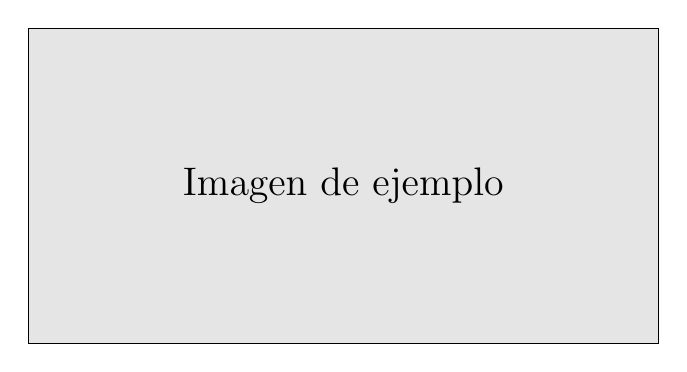
\begin{tikzpicture}
    \draw[fill=gray!20] (0,0) rectangle (8,4);
    \node at (4,2) {\Large Imagen de ejemplo};
  \end{tikzpicture}
  \caption{Ejemplo de figura simple (placeholder)}
  \label{fig:simple}
\end{figure}

Para referenciar la figura en el texto: ``como se muestra en la Figura~\ref{fig:simple}''.

\subsection{Opciones de includegraphics}
\label{subsec:opciones-includegraphics}

El comando \verb|\includegraphics| acepta múltiples opciones:

\begin{verbatim}
% Ancho relativo al texto
\includegraphics[width=0.8\textwidth]{imagen}

% Altura específica
\includegraphics[height=5cm]{imagen}

% Escala proporcional
\includegraphics[scale=0.5]{imagen}

% Rotar imagen
\includegraphics[angle=90]{imagen}

% Recortar imagen (izq, abajo, der, arriba)
\includegraphics[trim=1cm 2cm 1cm 2cm, clip]{imagen}

% Combinaciones
\includegraphics[width=0.6\textwidth, angle=45]{imagen}
\end{verbatim}

\subsection{Formatos de imagen soportados}
\label{subsec:formatos-imagen}

Con LuaLaTeX (el motor de esta plantilla) se soportan:
\begin{itemize}
  \item \textbf{PDF} --- Formato vectorial, ideal para diagramas y gráficas
  \item \textbf{PNG} --- Imágenes con transparencia
  \item \textbf{JPG/JPEG} --- Fotografías
  \item \textbf{EPS} --- PostScript encapsulado (convertido automáticamente)
\end{itemize}

\begin{tipbox}{Recomendación}
Usa PDF para gráficas vectoriales (exportadas desde Inkscape, MATLAB, Python) y PNG/JPG para fotografías. Evita formatos como BMP o TIFF.
\end{tipbox}

\subsection{Subfiguras}
\label{subsec:subfiguras}

Cuando necesitas mostrar varias imágenes relacionadas, usa el entorno \texttt{subfigure} del paquete \texttt{subcaption}:

\begin{verbatim}
\begin{figure}[H]
  \centering
  \begin{subfigure}[b]{0.45\textwidth}
    \centering
    \includegraphics[width=\textwidth]{imagen-a}
    \caption{Primera variante}
    \label{fig:sub-a}
  \end{subfigure}
  \hfill  % Espacio horizontal entre subfiguras
  \begin{subfigure}[b]{0.45\textwidth}
    \centering
    \includegraphics[width=\textwidth]{imagen-b}
    \caption{Segunda variante}
    \label{fig:sub-b}
  \end{subfigure}
  \caption{Título general de la figura}
  \label{fig:conjunto}
\end{figure}
\end{verbatim}

\begin{figure}[H]
  \centering
  \begin{subfigure}[b]{0.45\textwidth}
    \centering
    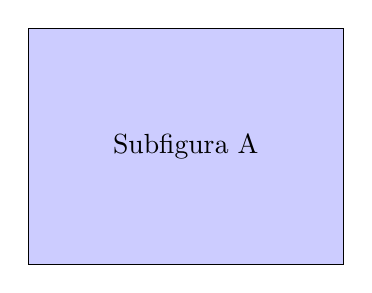
\begin{tikzpicture}
      \draw[fill=blue!20] (0,0) rectangle (4,3);
      \node at (2,1.5) {Subfigura A};
    \end{tikzpicture}
    \caption{Primera variante}
    \label{fig:sub-a}
  \end{subfigure}
  \hfill
  \begin{subfigure}[b]{0.45\textwidth}
    \centering
    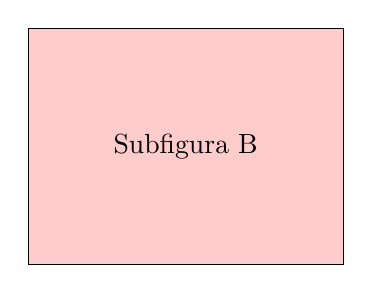
\begin{tikzpicture}
      \draw[fill=red!20] (0,0) rectangle (4,3);
      \node at (2,1.5) {Subfigura B};
    \end{tikzpicture}
    \caption{Segunda variante}
    \label{fig:sub-b}
  \end{subfigure}
  \caption{Ejemplo de subfiguras horizontales}
  \label{fig:subfiguras}
\end{figure}

Puedes referenciar subfiguras individuales: Figura~\ref{fig:sub-a} y Figura~\ref{fig:sub-b}, o el conjunto: Figura~\ref{fig:subfiguras}.

\subsection{Subfiguras verticales}
\label{subsec:subfiguras-verticales}

Para apilar subfiguras verticalmente, usa saltos de línea:

\begin{verbatim}
\begin{figure}[H]
  \centering
  \begin{subfigure}[b]{0.8\textwidth}
    \includegraphics[width=\textwidth]{imagen-arriba}
    \caption{Imagen superior}
  \end{subfigure}

  \vspace{0.5em}  % Espacio vertical

  \begin{subfigure}[b]{0.8\textwidth}
    \includegraphics[width=\textwidth]{imagen-abajo}
    \caption{Imagen inferior}
  \end{subfigure}
  \caption{Subfiguras apiladas verticalmente}
\end{figure}
\end{verbatim}

\subsection{Múltiples imágenes en cuadrícula}
\label{subsec:imagenes-cuadricula}

Para organizar varias imágenes en una cuadrícula, puedes usar un entorno \texttt{tabular} dentro de la figura:

\begin{verbatim}
\begin{figure}[H]
  \centering
  \begin{tabular}{ccc}
    \includegraphics[width=0.3\textwidth]{img1} &
    \includegraphics[width=0.3\textwidth]{img2} &
    \includegraphics[width=0.3\textwidth]{img3} \\
    Etiqueta 1 & Etiqueta 2 & Etiqueta 3 \\
  \end{tabular}
  \caption{Cuadrícula de imágenes}
\end{figure}
\end{verbatim}

\begin{figure}[H]
  \centering
  \begin{tabular}{ccc}
    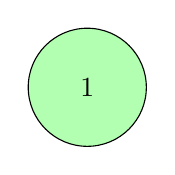
\begin{tikzpicture}[scale=0.5]
      \draw[fill=green!30] (0,0) circle (1.5);
      \node at (0,0) {1};
    \end{tikzpicture} &
    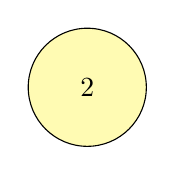
\begin{tikzpicture}[scale=0.5]
      \draw[fill=yellow!30] (0,0) circle (1.5);
      \node at (0,0) {2};
    \end{tikzpicture} &
    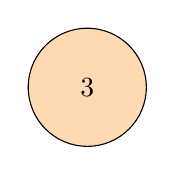
\begin{tikzpicture}[scale=0.5]
      \draw[fill=orange!30] (0,0) circle (1.5);
      \node at (0,0) {3};
    \end{tikzpicture} \\
    Config. A & Config. B & Config. C \\[1em]
    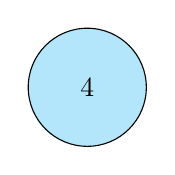
\begin{tikzpicture}[scale=0.5]
      \draw[fill=cyan!30] (0,0) circle (1.5);
      \node at (0,0) {4};
    \end{tikzpicture} &
    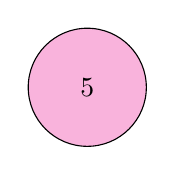
\begin{tikzpicture}[scale=0.5]
      \draw[fill=magenta!30] (0,0) circle (1.5);
      \node at (0,0) {5};
    \end{tikzpicture} &
    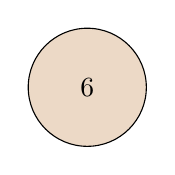
\begin{tikzpicture}[scale=0.5]
      \draw[fill=brown!30] (0,0) circle (1.5);
      \node at (0,0) {6};
    \end{tikzpicture} \\
    Config. D & Config. E & Config. F \\
  \end{tabular}
  \caption{Matriz de configuraciones experimentales}
  \label{fig:matriz}
\end{figure}

\section{Figuras a ancho completo}
\label{sec:figuras-ancho-meto}

Para figuras que ocupen todo el ancho de la página (incluyendo márgenes), usa el entorno \texttt{figure*} en documentos de dos columnas, o ajusta el ancho:

\begin{verbatim}
% Figura que ocupa todo el ancho del texto
\begin{figure}[H]
  \centering
  \includegraphics[width=\textwidth]{imagen-panoramica}
  \caption{Imagen a ancho completo}
\end{figure}

% Figura más ancha que el texto (sobresale en márgenes)
\begin{figure}[H]
  \centering
  \makebox[\textwidth][c]{%
    \includegraphics[width=1.2\textwidth]{imagen-extra-ancha}%
  }
  \caption{Imagen extra ancha}
\end{figure}
\end{verbatim}

\section{Planificación temporal}
\label{sec:planificacion-temporal}

La planificación temporal del proyecto se muestra en la Figura~\ref{fig:gantt}.

\begin{figure}[H]
  \centering
  \begin{tikzpicture}[
    fase/.style={fill=informatica!60, draw=informatica!80, rounded corners=2pt, minimum height=0.6cm},
    mes/.style={font=\footnotesize\sffamily},
    nombre/.style={font=\footnotesize, anchor=east}
  ]
    % Eje temporal (meses)
    \foreach \m/\n in {1/Sep, 2/Oct, 3/Nov, 4/Dic, 5/Ene, 6/Feb} {
      \node[mes] at (\m*1.5, 4.5) {\n};
    }

    % Líneas de guía verticales
    \foreach \m in {1,...,6} {
      \draw[gray!30] (\m*1.5-0.75, 0.5) -- (\m*1.5-0.75, 4);
    }

    % Fases del proyecto
    \node[nombre] at (0, 3.5) {Análisis};
    \draw[fase] (0.75, 3.3) rectangle (2.25, 3.7);

    \node[nombre] at (0, 2.8) {Diseño};
    \draw[fase] (1.5, 2.6) rectangle (3.75, 3);

    \node[nombre] at (0, 2.1) {Implementación};
    \draw[fase] (3, 1.9) rectangle (6.75, 2.3);

    \node[nombre] at (0, 1.4) {Pruebas};
    \draw[fase] (5.25, 1.2) rectangle (7.5, 1.6);

    \node[nombre] at (0, 0.7) {Documentación};
    \draw[fase] (6, 0.5) rectangle (9, 0.9);
  \end{tikzpicture}
  \caption{Planificación temporal del proyecto (diagrama de Gantt simplificado)}
  \label{fig:gantt}
\end{figure}

\section{Diagramas con TikZ}
\label{sec:diagramas-tikz}

TikZ es un paquete muy potente para crear diagramas vectoriales directamente en \LaTeX{}. A diferencia de las imágenes importadas, los diagramas TikZ se escalan perfectamente y usan las mismas fuentes del documento.

\subsection{Diagrama de flujo}
\label{subsec:diagrama-flujo-metodo}

Los diagramas de flujo son esenciales para documentar algoritmos y procesos:

\begin{figure}[H]
  \centering
  \begin{tikzpicture}[
    node distance=1.5cm,
    startstop/.style={rectangle, rounded corners, minimum width=2.5cm, minimum height=0.8cm, text centered, draw=black, fill=red!30},
    process/.style={rectangle, minimum width=2.5cm, minimum height=0.8cm, text centered, draw=black, fill=blue!20},
    decision/.style={diamond, minimum width=2cm, minimum height=0.8cm, text centered, draw=black, fill=green!20, aspect=2},
    arrow/.style={thick,->,>=stealth}
  ]
    \node (start) [startstop] {Inicio};
    \node (proc1) [process, below of=start] {Proceso 1};
    \node (dec1) [decision, below of=proc1, yshift=-0.5cm] {¿Condición?};
    \node (proc2) [process, below of=dec1, yshift=-0.5cm] {Proceso 2};
    \node (proc3) [process, right of=dec1, xshift=2cm] {Alternativa};
    \node (stop) [startstop, below of=proc2] {Fin};

    \draw [arrow] (start) -- (proc1);
    \draw [arrow] (proc1) -- (dec1);
    \draw [arrow] (dec1) -- node[anchor=east] {Sí} (proc2);
    \draw [arrow] (dec1) -- node[anchor=south] {No} (proc3);
    \draw [arrow] (proc3) |- (proc2);
    \draw [arrow] (proc2) -- (stop);
  \end{tikzpicture}
  \caption{Diagrama de flujo del algoritmo principal}
  \label{fig:flowchart}
\end{figure}

\subsection{Diagrama de bloques}
\label{subsec:diagrama-bloques-metodo}

Los diagramas de bloques son útiles para representar arquitecturas de sistemas:

\begin{figure}[H]
  \centering
  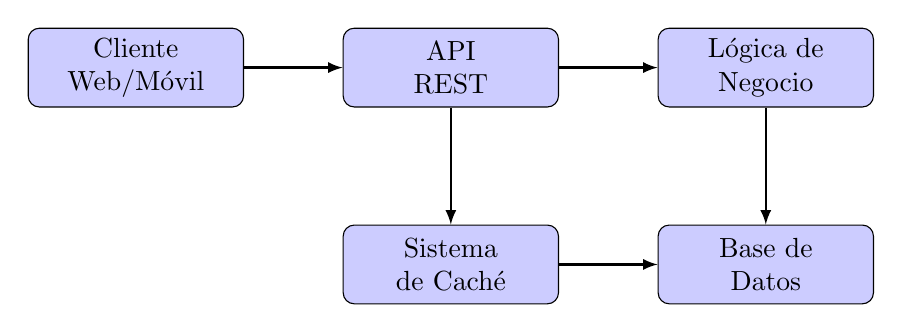
\begin{tikzpicture}[
    block/.style={rectangle, draw, fill=blue!20, text width=2.5cm, text centered, rounded corners, minimum height=1cm},
    line/.style={draw, thick, -latex}
  ]
    \node [block] (cliente) {Cliente\\Web/Móvil};
    \node [block, right of=cliente, xshift=3cm] (api) {API\\REST};
    \node [block, right of=api, xshift=3cm] (logica) {Lógica de\\Negocio};
    \node [block, below of=logica, yshift=-1.5cm] (bd) {Base de\\Datos};
    \node [block, below of=api, yshift=-1.5cm] (cache) {Sistema\\de Caché};

    \path [line] (cliente) -- (api);
    \path [line] (api) -- (logica);
    \path [line] (logica) -- (bd);
    \path [line] (api) -- (cache);
    \path [line] (cache) -- (bd);
  \end{tikzpicture}
  \caption{Arquitectura del sistema}
  \label{fig:arquitectura-metodo}
\end{figure}

\section{Buenas prácticas con figuras}
\label{sec:buenas-practicas-figuras}

A continuación se resumen las recomendaciones para trabajar con figuras en documentos académicos:

\begin{infobox}{Convenciones de nombrado}
Usa prefijos consistentes para las etiquetas: \texttt{fig:} para figuras, \texttt{tab:} para tablas, \texttt{eq:} para ecuaciones, \texttt{sec:} para secciones.
\end{infobox}

\subsection{Organización de archivos}
\label{subsec:organizacion-archivos}

Se recomienda organizar las imágenes en carpetas dentro de \texttt{recursos/}:

\begin{verbatim}
recursos/
├── imagenes/
│   ├── capturas/       % Capturas de pantalla
│   ├── diagramas/      % Diagramas exportados
│   ├── fotografias/    % Fotos del proyecto
│   └── graficas/       % Gráficas de datos
└── logos/              % Logotipos institucionales
\end{verbatim}

\subsection{Calidad de las imágenes}
\label{subsec:calidad-imagenes}

\begin{itemize}
  \item \textbf{Resolución mínima:} 300 DPI para impresión
  \item \textbf{Formato vectorial:} Preferir PDF para diagramas y gráficas
  \item \textbf{Tamaño de archivo:} Optimizar imágenes grandes antes de incluirlas
  \item \textbf{Consistencia:} Usar el mismo estilo visual en todas las figuras
\end{itemize}

\subsection{Texto en figuras}
\label{subsec:texto-figuras}

El texto dentro de las figuras debe ser legible cuando se imprima:

\begin{warningbox}{Tamaño mínimo de texto}
El texto en figuras debe tener al menos 8pt cuando se muestren al tamaño final. Evita texto demasiado pequeño que resulte ilegible.
\end{warningbox}

\section{Recursos utilizados}
\label{sec:recursos-utilizados}

\subsection{Recursos hardware}
\label{subsec:recursos-hardware}

\begin{itemize}
  \item Ordenador portátil con procesador Intel i7, 16GB RAM
  \item Servidor de desarrollo con 32GB RAM
  \item Dispositivos móviles para pruebas
\end{itemize}

\subsection{Recursos software}
\label{subsec:recursos-software}

\begin{itemize}
  \item Sistema operativo: Linux Ubuntu 24.04 LTS
  \item Entorno de desarrollo: Visual Studio Code
  \item Control de versiones: Git y GitHub
  \item Compilador \LaTeX{}: LuaLaTeX (TeX Live 2024)
\end{itemize}

\section{Gestión del proyecto}
\label{sec:gestion-proyecto}

Para la gestión del proyecto se han utilizado las siguientes herramientas:

\begin{itemize}
  \item \textbf{GitHub Projects:} Para la gestión de tareas y seguimiento del progreso mediante tableros Kanban.
  \item \textbf{Git:} Para el control de versiones del código y la documentación.
  \item \textbf{Discord/Slack:} Para la comunicación con el tutor.
\end{itemize}

\section{Resumen de comandos para figuras}
\label{sec:resumen-comandos-figuras}

A modo de referencia rápida, estos son los comandos más utilizados:

\begin{verbatim}
% Figura básica
\begin{figure}[H]
  \centering
  \includegraphics[width=0.8\textwidth]{ruta/imagen}
  \caption{Título de la figura}
  \label{fig:etiqueta}
\end{figure}

% Referenciar figura
Ver Figura~\ref{fig:etiqueta}

% Subfiguras (requiere subcaption)
\begin{subfigure}[b]{0.45\textwidth}
  ...
\end{subfigure}

% Opciones comunes de includegraphics
width=      % Ancho (ej: 0.8\textwidth, 10cm)
height=     % Alto
scale=      % Escala (ej: 0.5)
angle=      % Rotación en grados
trim=       % Recorte: izq abajo der arriba
clip        % Activar recorte
\end{verbatim}
